
%% bare_conf.tex
%% V1.4b
%% 2015/08/26
%% by Michael Shell
%% See:
%% http://www.michaelshell.org/
%% for current contact information.
%%
%% This is a skeleton file demonstrating the use of IEEEtran.cls
%% (requires IEEEtran.cls version 1.8b or later) with an IEEE
%% conference paper.
%%
%% Support sites:
%% http://www.michaelshell.org/tex/ieeetran/
%% http://www.ctan.org/pkg/ieeetran
%% and
%% http://www.ieee.org/

%%*************************************************************************
%% Legal Notice:
%% This code is offered as-is without any warranty either expressed or
%% implied; without even the implied warranty of MERCHANTABILITY or
%% FITNESS FOR A PARTICULAR PURPOSE! 
%% User assumes all risk.
%% In no event shall the IEEE or any contributor to this code be liable for
%% any damages or losses, including, but not limited to, incidental,
%% consequential, or any other damages, resulting from the use or misuse
%% of any information contained here.
%%
%% All comments are the opinions of their respective authors and are not
%% necessarily endorsed by the IEEE.
%%
%% This work is distributed under the LaTeX Project Public License (LPPL)
%% ( http://www.latex-project.org/ ) version 1.3, and may be freely used,
%% distributed and modified. A copy of the LPPL, version 1.3, is included
%% in the base LaTeX documentation of all distributions of LaTeX released
%% 2003/12/01 or later.
%% Retain all contribution notices and credits.
%% ** Modified files should be clearly indicated as such, including  **
%% ** renaming them and changing author support contact information. **
%%*************************************************************************


% *** Authors should verify (and, if needed, correct) their LaTeX system  ***
% *** with the testflow diagnostic prior to trusting their LaTeX platform ***
% *** with production work. The IEEE's font choices and paper sizes can   ***
% *** trigger bugs that do not appear when using other class files.       ***                          ***
% The testflow support page is at:
% http://www.michaelshell.org/tex/testflow/



\documentclass[conference]{IEEEtran}
% Some Computer Society conferences also require the compsoc mode option,
% but others use the standard conference format.
%
% If IEEEtran.cls has not been installed into the LaTeX system files,
% manually specify the path to it like:
% \documentclass[conference]{../sty/IEEEtran}

\IEEEoverridecommandlockouts



% Some very useful LaTeX packages include:
% (uncomment the ones you want to load)


% *** MISC UTILITY PACKAGES ***
%
%\usepackage{ifpdf}
% Heiko Oberdiek's ifpdf.sty is very useful if you need conditional
% compilation based on whether the output is pdf or dvi.
% usage:
% \ifpdf
%   % pdf code
% \else
%   % dvi code
% \fi
% The latest version of ifpdf.sty can be obtained from:
% http://www.ctan.org/pkg/ifpdf
% Also, note that IEEEtran.cls V1.7 and later provides a builtin
% \ifCLASSINFOpdf conditional that works the same way.
% When switching from latex to pdflatex and vice-versa, the compiler may
% have to be run twice to clear warning/error messages.






% *** CITATION PACKAGES ***
%
%\usepackage{cite}
% cite.sty was written by Donald Arseneau
% V1.6 and later of IEEEtran pre-defines the format of the cite.sty package
% \cite{} output to follow that of the IEEE. Loading the cite package will
% result in citation numbers being automatically sorted and properly
% "compressed/ranged". e.g., [1], [9], [2], [7], [5], [6] without using
% cite.sty will become [1], [2], [5]--[7], [9] using cite.sty. cite.sty's
% \cite will automatically add leading space, if needed. Use cite.sty's
% noadjust option (cite.sty V3.8 and later) if you want to turn this off
% such as if a citation ever needs to be enclosed in parenthesis.
% cite.sty is already installed on most LaTeX systems. Be sure and use
% version 5.0 (2009-03-20) and later if using hyperref.sty.
% The latest version can be obtained at:
% http://www.ctan.org/pkg/cite
% The documentation is contained in the cite.sty file itself.






% *** GRAPHICS RELATED PACKAGES ***
%
\ifCLASSINFOpdf
   \usepackage[pdftex]{graphicx}
  % declare the path(s) where your graphic files are
   \graphicspath{{./figs/}}
  % and their extensions so you won't have to specify these with
  % every instance of \includegraphics
   \DeclareGraphicsExtensions{.pdf,.jpeg,.png}
\else
  % or other class option (dvipsone, dvipdf, if not using dvips). graphicx
  % will default to the driver specified in the system graphics.cfg if no
  % driver is specified.
  % \usepackage[dvips]{graphicx}
  % declare the path(s) where your graphic files are
  % \graphicspath{{../eps/}}
  % and their extensions so you won't have to specify these with
  % every instance of \includegraphics
  % \DeclareGraphicsExtensions{.eps}
\fi
% graphicx was written by David Carlisle and Sebastian Rahtz. It is
% required if you want graphics, photos, etc. graphicx.sty is already
% installed on most LaTeX systems. The latest version and documentation
% can be obtained at: 
% http://www.ctan.org/pkg/graphicx
% Another good source of documentation is "Using Imported Graphics in
% LaTeX2e" by Keith Reckdahl which can be found at:
% http://www.ctan.org/pkg/epslatex
%
% latex, and pdflatex in dvi mode, support graphics in encapsulated
% postscript (.eps) format. pdflatex in pdf mode supports graphics
% in .pdf, .jpeg, .png and .mps (metapost) formats. Users should ensure
% that all non-photo figures use a vector format (.eps, .pdf, .mps) and
% not a bitmapped formats (.jpeg, .png). The IEEE frowns on bitmapped formats
% which can result in "jaggedy"/blurry rendering of lines and letters as
% well as large increases in file sizes.
%
% You can find documentation about the pdfTeX application at:
% http://www.tug.org/applications/pdftex





% *** MATH PACKAGES ***
%
%\usepackage{amsmath}
% A popular package from the American Mathematical Society that provides
% many useful and powerful commands for dealing with mathematics.
%
% Note that the amsmath package sets \interdisplaylinepenalty to 10000
% thus preventing page breaks from occurring within multiline equations. Use:
%\interdisplaylinepenalty=2500
% after loading amsmath to restore such page breaks as IEEEtran.cls normally
% does. amsmath.sty is already installed on most LaTeX systems. The latest
% version and documentation can be obtained at:
% http://www.ctan.org/pkg/amsmath





% *** SPECIALIZED LIST PACKAGES ***
%
%\usepackage{algorithmic}
% algorithmic.sty was written by Peter Williams and Rogerio Brito.
% This package provides an algorithmic environment fo describing algorithms.
% You can use the algorithmic environment in-text or within a figure
% environment to provide for a floating algorithm. Do NOT use the algorithm
% floating environment provided by algorithm.sty (by the same authors) or
% algorithm2e.sty (by Christophe Fiorio) as the IEEE does not use dedicated
% algorithm float types and packages that provide these will not provide
% correct IEEE style captions. The latest version and documentation of
% algorithmic.sty can be obtained at:
% http://www.ctan.org/pkg/algorithms
% Also of interest may be the (relatively newer and more customizable)
% algorithmicx.sty package by Szasz Janos:
% http://www.ctan.org/pkg/algorithmicx




% *** ALIGNMENT PACKAGES ***
%
%\usepackage{array}
% Frank Mittelbach's and David Carlisle's array.sty patches and improves
% the standard LaTeX2e array and tabular environments to provide better
% appearance and additional user controls. As the default LaTeX2e table
% generation code is lacking to the point of almost being broken with
% respect to the quality of the end results, all users are strongly
% advised to use an enhanced (at the very least that provided by array.sty)
% set of table tools. array.sty is already installed on most systems. The
% latest version and documentation can be obtained at:
% http://www.ctan.org/pkg/array


% IEEEtran contains the IEEEeqnarray family of commands that can be used to
% generate multiline equations as well as matrices, tables, etc., of high
% quality.




% *** SUBFIGURE PACKAGES ***
%\ifCLASSOPTIONcompsoc
%  \usepackage[caption=false,font=normalsize,labelfont=sf,textfont=sf]{subfig}
%\else
%  \usepackage[caption=false,font=footnotesize]{subfig}
%\fi
% subfig.sty, written by Steven Douglas Cochran, is the modern replacement
% for subfigure.sty, the latter of which is no longer maintained and is
% incompatible with some LaTeX packages including fixltx2e. However,
% subfig.sty requires and automatically loads Axel Sommerfeldt's caption.sty
% which will override IEEEtran.cls' handling of captions and this will result
% in non-IEEE style figure/table captions. To prevent this problem, be sure
% and invoke subfig.sty's "caption=false" package option (available since
% subfig.sty version 1.3, 2005/06/28) as this is will preserve IEEEtran.cls
% handling of captions.
% Note that the Computer Society format requires a larger sans serif font
% than the serif footnote size font used in traditional IEEE formatting
% and thus the need to invoke different subfig.sty package options depending
% on whether compsoc mode has been enabled.
%
% The latest version and documentation of subfig.sty can be obtained at:
% http://www.ctan.org/pkg/subfig




% *** FLOAT PACKAGES ***
%
%\usepackage{fixltx2e}
% fixltx2e, the successor to the earlier fix2col.sty, was written by
% Frank Mittelbach and David Carlisle. This package corrects a few problems
% in the LaTeX2e kernel, the most notable of which is that in current
% LaTeX2e releases, the ordering of single and double column floats is not
% guaranteed to be preserved. Thus, an unpatched LaTeX2e can allow a
% single column figure to be placed prior to an earlier double column
% figure.
% Be aware that LaTeX2e kernels dated 2015 and later have fixltx2e.sty's
% corrections already built into the system in which case a warning will
% be issued if an attempt is made to load fixltx2e.sty as it is no longer
% needed.
% The latest version and documentation can be found at:
% http://www.ctan.org/pkg/fixltx2e


%\usepackage{stfloats}
% stfloats.sty was written by Sigitas Tolusis. This package gives LaTeX2e
% the ability to do double column floats at the bottom of the page as well
% as the top. (e.g., "\begin{figure*}[!b]" is not normally possible in
% LaTeX2e). It also provides a command:
%\fnbelowfloat
% to enable the placement of footnotes below bottom floats (the standard
% LaTeX2e kernel puts them above bottom floats). This is an invasive package
% which rewrites many portions of the LaTeX2e float routines. It may not work
% with other packages that modify the LaTeX2e float routines. The latest
% version and documentation can be obtained at:
% http://www.ctan.org/pkg/stfloats
% Do not use the stfloats baselinefloat ability as the IEEE does not allow
% \baselineskip to stretch. Authors submitting work to the IEEE should note
% that the IEEE rarely uses double column equations and that authors should try
% to avoid such use. Do not be tempted to use the cuted.sty or midfloat.sty
% packages (also by Sigitas Tolusis) as the IEEE does not format its papers in
% such ways.
% Do not attempt to use stfloats with fixltx2e as they are incompatible.
% Instead, use Morten Hogholm'a dblfloatfix which combines the features
% of both fixltx2e and stfloats:
%
% \usepackage{dblfloatfix}
% The latest version can be found at:
% http://www.ctan.org/pkg/dblfloatfix




% *** PDF, URL AND HYPERLINK PACKAGES ***
%
\usepackage{url}
% url.sty was written by Donald Arseneau. It provides better support for
% handling and breaking URLs. url.sty is already installed on most LaTeX
% systems. The latest version and documentation can be obtained at:
% http://www.ctan.org/pkg/url
% Basically, \url{my_url_here}.




% *** Do not adjust lengths that control margins, column widths, etc. ***
% *** Do not use packages that alter fonts (such as pslatex).         ***
% There should be no need to do such things with IEEEtran.cls V1.6 and later.
% (Unless specifically asked to do so by the journal or conference you plan
% to submit to, of course. )


% correct bad hyphenation here
\hyphenation{op-tical net-works semi-conduc-tor}
 

\begin{document}
%
% paper title
% Titles are generally capitalized except for words such as a, an, and, as,
% at, but, by, for, in, nor, of, on, or, the, to and up, which are usually
% not capitalized unless they are the first or last word of the title.
% Linebreaks \\ can be used within to get better formatting as desired.
% Do not put math or special symbols in the title.
\title{Causal Inference for ATM Counterfactual Estimation}


% author names and affiliations
% use a multiple column layout for up to three different
% affiliations
\author{\IEEEauthorblockN{Akhil Shah}
\IEEEauthorblockA{RAND Corporation\\
Santa Monica, CA 90407\\
Email: ashah@rand.org}
}

% conference papers do not typically use \thanks and this command
% is locked out in conference mode. If really needed, such as for
% the acknowledgment of grants, issue a \IEEEoverridecommandlockouts
% after \documentclass

% for over three affiliations, or if they all won't fit within the width
% of the page, use this alternative format:
% 
%\author{\IEEEauthorblockN{Michael Shell\IEEEauthorrefmark{1},
%Homer Simpson\IEEEauthorrefmark{2},
%James Kirk\IEEEauthorrefmark{3}, 
%Montgomery Scott\IEEEauthorrefmark{3} and
%Eldon Tyrell\IEEEauthorrefmark{4}}
%\IEEEauthorblockA{\IEEEauthorrefmark{1}School of Electrical and Computer Engineering\\
%Georgia Institute of Technology,
%Atlanta, Georgia 30332--0250\\ Email: see http://www.michaelshell.org/contact.html}
%\IEEEauthorblockA{\IEEEauthorrefmark{2}Twentieth Century Fox, Springfield, USA\\
%Email: homer@thesimpsons.com}
%\IEEEauthorblockA{\IEEEauthorrefmark{3}Starfleet Academy, San Francisco, California 96678-2391\\
%Telephone: (800) 555--1212, Fax: (888) 555--1212}
%\IEEEauthorblockA{\IEEEauthorrefmark{4}Tyrell Inc., 123 Replicant Street, Los Angeles, California 90210--4321}}




% use for special paper notices
%\IEEEspecialpapernotice{(Invited Paper)}




% make the title area
\maketitle

% As a general rule, do not put math, special symbols or citations
% in the abstract
\begin{abstract}
We propose that the Rubin potential outcomes framework of causal inference can be used to statistically estimate counterfactuals, by definition never observable, of Traffic Flow Management Initiatives (TFMI), as a novel means of quantifying performance Air Traffic Management (ATM) actions, despite confounding factors.  Specifically, we apply the method of Propensity Scores to estimate counterfactuals and compute the increase in hourly average airborne delay which would have resulted without a Ground Delay Program, using an eleven month span of hourly weather, traffic, and delay data at JFK.   Our introduction also summarizes the concepts of causal inference required for our analysis.   We also offer suggestions to improve and extend our initial application of casual inference.  Technical details of propensity score modeling are further covered in an appendix.
\end{abstract}

% no keywords

\begin{IEEEkeywords}
ATM Performance Measurement, Causal Inference, Propensity Scores
\end{IEEEkeywords}



% For peer review papers, you can put extra information on the cover
% page as needed:
% \ifCLASSOPTIONpeerreview
% \begin{center} \bfseries EDICS Category: 3-BBND \end{center}
% \fi
%
% For peerreview papers, this IEEEtran command inserts a page break and
% creates the second title. It will be ignored for other modes.
\IEEEpeerreviewmaketitle



\section{Introduction}
% no \IEEEPARstart
%The Federal Aviation Administration (FAA) is the governmental agency responsible for policy and oversight of air transportation in the United States.  Many day-to-day Air Traffic Management (ATM) decisions are made by the Air Traffic Control System Command Center (ATCSCC), which has ``final approval authority for all national traffic management initiatives."  The ATCSCC implements its authority by publishing timely Air Traffic Flow Management Initiatives (ATFMI), regularly consulting with Airline Operation Centers (AOC) using a process known as Collaborative Decision Making.   

%Both the ATCSCC and AOC regularly implement ATFMI, such as Ground Delay Programs (GDP), which purposefully delay flights on the ground at the departure airport to avoid more costly and less safe airborne delays at the arrival airport.  Other examples of ATFMI include Ground Stops and Reroutes\footnote{More examples of ATFMI and detailed descriptions can be found in \cite{faatfm}.}.  These initiatives increase the safety and efficiency of the nation's air transportation system, for example replacing airborne delay with ground delay, and are necessary during inclement weather and in other situations where demand exceeds various capacities, such as airport arrival capacity.  The complexity of optimally allocating constrained resources have motivated researchers to develop decision making aids, for example \cite{pyrgiotis2011public}, that can assist operators to evaluate tradeoffs of available ATFMI.

Traffic managers at the Air Traffic Control System Command Center (ATCSCC) and other stakeholders, such the Airlines Operations Centers (AOC), should be able to estimate performance metrics, such as ground and airborne delays, due to various courses of actions. Moreover, improvements in Air Traffic Management (ATM) require accurate estimates of actual and potential outcomes of specific Traffic Flow Management Initiatives (TFMI), interventions which ensure and enhance performance of the National Air Space, in order to enable comparison of  alternative courses of actions.  These performance estimates of alternative courses of action can result from simulation or statistical inference.  Thus motivated, we present a novel application of a well developed statistical methodology, causal inference, which enables estimating the effectiveness of interventions, such as TFMI, through constructing counterfactual outcomes, by definition never observable, and has been useful in various other domains where random trials are impractical, including health \cite{austin2011tutorial,victora2004evidence}, economics \cite{bottou2013counterfactual,tariq2009detecting} and ecological contexts\footnote{For example: \url{https://www3.epa.gov/caddis/da_advanced_5.html}}.  However, to the best of our knowledge, casual inference has not yet been explored in the ATM research community.  We argue that causal inference may provide a statistically rigorous framework to estimate the effectiveness of TFMI, despite the presence of \emph{confounding} in ATM datasets.  

In addition to summarizing the conceptual aspects of causal inference, we will illustrate a specific ATM use case: estimating the potential outcome of not implementing a particular TFMI, namely the potential airborne delay which if a Ground Delay Programs (GDP) had not been implemented during hours when it was in fact implemented at JFK.  

\subsection{Confounding in ATM Data}
Consider the case of evaluating the efficacy of a medical treatment.  One option is to implement randomized control trials, where units are randomly assigned to treatment and control groups, and is sometimes feasible.  However randomized control trials, considered the gold-standard to statistically evaluate the effectiveness of a treatment \cite{austin2011introduction}, are not always possible to implement.  For example, lets consider the efficacy of smoking cessation counseling for smokers admitted to a hospital for a heart attack \cite{austin2011tutorial}.  In particular, we are interested in the following question: does smoking cessation counseling, prior to discharge from the hospital, increase the lifespan of smokers who have suffered a heart attack?  If a randomized control trial were possible in this situation, then the usual methods of regression would suffice to answer this question statistically.  However there are various barriers to voluntary participation and completion of treatment \cite{austin2011tutorial}, and thus a random controlled experiment is not possible in this example.  Statisticians call such a situation an ``observational study," and commonly, there are systematic differences between patients who receive treatment and those who do not, which must be accounted for in a sound methodological manner when assessing the effect of a treatment on the outcome of interest (e.g. mortality). 

Similarly, in the ATM context, it is infeasible to conduct randomized control trials.  For a particular TFMI, such as a Ground Delay Program (GDP), blocks of time or individual flights are clearly not assigned randomly to the initiative, but are the consequence of a collaborative decision making process based on various factors such as weather, traffic, and capacity.  Furthermore, outcomes, such as airborne delay are also influenced by these same covariates; hours of inclement weather are more likely to be assigned GDP and they are also likely to experience higher average airborne delay than hours with clear weather.  Thus to empirically estimate the effectiveness of a TFMI like GDP requires accounting for these confounding factors.

Estimates of performance metrics can enable tradeoffs between different courses of action.  More specifically, counterfactual estimates of performance due to a given TFMI,  can provide decision makers an estimate of the potential cost of inaction, for example average airborne delays if a GDP had not been imposed at a given arrival airport.  These counterfactual estimates may be useful both at operational and strategic levels when evaluating the cost and benefits of various TFMI at various spatial and temporal scales.  However estimating counterfactual outcomes is methodologically challenging in the ATM context where the notion of random trials or random assignment of flights to  is impractical.  We propose to employ the statistical methodology of causal inference to derive these counterfactual estimates, which have the advantage of being derived from a statistically rigorous framework that has been applied in various other domains, such as health, education, and economics.  To our knowledge, this is the first application of causal inference to ATM.  

As explained in \cite{austin2011introduction}, the fundamental difficulty of observational studies versus random controlled trials, is the presence of \emph{confounding}:  the outcome of interest (e.g. mortality) is influenced by both the treatment status (i.e. whether the patient received or did not receive treatment) and the baseline characteristics, which are often systematically different between the treatment and control groups.  Although there exist regression adjustment techniques that attempt to account for confounding, there are many reasons for which they are not robust \cite{austin2011introduction,austin2011tutorial,mccaffrey2013tutorial}.  An alternative method to eliminate or reduce confounding uses the idea of propensity scores and the potential outcomes framework on which they are based.

\subsection{Related research}
Various approaches can be used to analyze alternative courses of actions for ATM.  One possibility is to use a dynamic systems modeling approach, employing a combination of analytic models and discrete-event simulations.  Tools such as ACES and FACET \cite{facet} can be used to simulate airborne delay statistics from various TFMI implementation strategies with realistic traffic flows.  Queuing theoretic models, with varying degrees of simplifications, can also be used to to analyze delay statistics resulting from a range of GDP implementation parameters \cite{ball2001analysis,kim2009air,sengupta2010computational,gwiggner2014data, caccavale2014model}. 

%\footnote{Examples of other NAS capacity modeling tools can be found at: \url{http://onlinepubs.trb.org/Onlinepubs/circulars/ec042/04_Donohue.pdf}} %

Alternatively one can use techniques that don't directly model the dynamics of weather and traffic in the NAS through analytic or discrete-event approaches, but rather through statistical techniques for producing \emph{counterfactual} scenarios unobserved in the historical data.  These counterfactual scenarios can then be used to estimate the impact of potential TFMI given weather and traffic forecasts and thus aid 'what-if' analysis required of decision makers.  For example \cite{kim2013} uses a statistical simulation technique (``quantile equivalence") to generate counterfactual scenarios of demand and throughput at LGA, EWR, and JFK, and consequently predicts delay at these airports.  This method does account for a single, but relevant, weather feature using an empirical non-parametric procedure to statistically simulate counterfactual scenarios by mixing \emph{observed} throughput and demand in various time periods for a given weather condition (either VMC or IMC).  


\subsection{Outline}
In this report we will examine another approach, Causal Inference, to generate counterfactual estimates, which can additionally quantify and reduce confounding, in order to attribute effectiveness of interventions (like TFMI) in terms of relevant outcomes. Causal Inference actually comprises several statistical methods, including propensity scores \cite{austin2011tutorial}, which we will specifically employ for counterfactual estimation to evaluate TFMI impact on system outcomes in the presence of confounding factors such as weather and demand.

Our initial examination of airborne delay under a GDP is the simplest application of Causal Inference, using hourly data as the unit of analysis, with binary treatment assignment (GDP or no GDP).  In our conclusions, we offer the ATM research community various possible extensions of our initial application of Causal Inference. We will briefly discuss more sophsiticated possibilities employing other units of analysis, such as individual flights, multiple discrete treatments for GDP across multiple airports, and continuous treatment variables such as the amount of ground delay.  We will also articulate the various challenges which accompany such an undertaking in our conclusion.  

\section{Essential Concepts of Causal Inference}
\subsection{Potential Outcomes}
The Rubin potential outcomes framework \cite{rubin1974estimating} imagines two possible treatment assignments for each unit of analysis (e.g. a patient, a flight, or a block of time), i.e. a treatment and control, and denotes the treatment status for each unit with the indicator variable $Z$ ($Z=0$ for control and $Z=1$ for treatment).  For each unit, the effect of the treatment on the outcome (e.g. mortality, delay, etc.) $Y$ is defined to be $Y_i(Z=1) - Y_i(Z=0)$.  Notice however that for each unit, only one reality is observed, and thus to compute effect, we must be able to statistically estimate the counterfactual or potential outcome.  For example, for a subject who ultimately receives treatment, we can only observe $Y_i(Z=1)$, but not the counterfactual $Y_i(Z=0)$.  The potential outcomes framework attempts to estimate counterfactuals so that the average effect of the treatment can be computed either for all subjects, called the average treatment effect (ATE),  or for only the subject that received treatment, called the average treatment effect on the treated (ATT).  Note that the analyst must decide which quantity is more appropriate to estimate; for example in the smoking cessation counseling example, ATT is the appropriate quantity to estimate as it is not realistic that all patients would likely elect treatment \cite{austin2011tutorial}.  However if the treatment were instead a brochure on smoking, the barrier to treatment entry is low, and thus ATE would be appropriate to estimate as it is realistic to assume that all subjects could potentially be part of either treatment or control group.  We argue  that in our context of TFMI ``treatments" (e.g. GDP), ATT is the more appropriate quantity to estimate, because it is unrealistic to assume that all time-periods (e.g. even those with ``good" weather and normal traffic and capacity characteristics) would potentially be subject to TFMI action.  Also note that to calculate ATT, $E[Y(Z=1) - Y(Z=0)| Z=1]$, we only need to estimate the counterfactual for units in the treatment group (i.e. estimate the counterfactual Y(Z=0) for the treated subjects), whereas for ATE, the counterfactual for the control group must also be estimated.  

In the next section we explain how confounding can be reduced by balancing the baseline characteristics using the propensity score.  The aim of balancing pretreatment covariates can also be viewed as transforming data from an observational study so it resembles the gold standard of a randomized control trial \cite{austin2011introduction}.  

\subsection{Propensity Score}
The propensity score is defined as $e_i=Pr(Z_i=1|X_i)$, namely the \emph{probability} that subject $i$ with baseline characteristics described by the covariate vector $X_i$ is assigned to the treatment group.  Note that all subjects have a propensity score in the potential outcomes framework, regardless of whether they were actually in the treatment or control group.  The important statistical property of the propensity score is that it is a \emph{balancing score} \cite{austin2011introduction}: conditional on the propensity score, the distribution of baseline covariates is similar between treated and control subjects.  Thus for a set of subjects with the same propensity score (value of $e_i$), there should be no statistically significant difference in baseline covariates, and thus a counterfactual outcome can be estimated, allowing the eventual estimate of ATT or ATE.  

Thus far we have summarized the fundamental obstruction to causal analysis in observational studies, namely confounding, and have also reviewed how the potential outcomes framework and counterfactual estimation can be used in principal to overcome confounding, and how the propensity score's balancing property can provide such counterfactual estimation\footnote{See \cite{austin2011introduction} for the further discussion on statistical assumptions that underly the balancing property of propensity scores and which allow confounding to be reduced or eliminated}. In the appendix, we clarify the mechanics of how propensity scores are estimated, namely the various model and the model fitting procedures, and how the scores are then used to balance covariates and estimate ATE or ATT using various methods. 

Our application of the potential outcomes framework using propensity scores to estimate the impact of potential TFMI uses the following analogy: each record is an hour time period at a given airport; measured baseline characteristics are historical forecasts of weather (relevant features from TAF) and traffic (hourly arrival data from ASPM); treatment assignment is the occurrence of a TFMI in the time period (such as GDP); and measured outcome is the hourly averaged airborne delay, also recorded in ASPM.  



\section{Application to GDP}
TFMI are designed to increase the safety and efficiency of the nation's air transportation system, and are necessary during inclement weather and in other situations where demand exceeds capacity.  When the arrival capacity of airport cannot accommodate demand, either due to weather induced diminished capacity or volume induced enhanced demand, a GDP is often implemented.  A GDP will purposefully delay flights on the ground at the various origin airports to avoid more costly airborne delays that would be incurred at the arrival airport\footnote{Further examples of TFMI and detailed descriptions can be found in \cite{faatfm}.}. Designing a GDP involves setting a planned airport acceptance rate (PAAR), commensurate with the forecasted arrival capacity, and then sequencing affected flights with controlled departure times, ideally with an equitable distribution of delays \cite{ball2001analysis}.  Increasing or decreasing this PAAR, or inversely the inter-arrival time between flights, transfers the overall delay of all flights subject to the GDP between airborne or ground portions (higher PAAR means more of the overall delay is absorbed in the air).  

Our causal analysis will specifically focus on estimating the counterfactual outcomes of a GDP at JFK, using a variety of data sources, to be detailed shortly, that span eleven months between October 2013 and September 2014. As noticed in \cite{bilimoria2016analysis}, the average airborne delay for flights with GDP ground-delays is roughly four minutes larger than the average airborne delays for flights that did not receive an EDCT under a GDP.  However it is commonly understood that in absence of a GDP, namely the counterfactual of not applying  ground-delay to the affected flights, the arrival airport would experience even larger airborne delays than actually observed in reality.  In terms of a queuing model \cite{ball2001analysis}, not instituting a GDP during diminished arrival capacity or enhanced traffic volume, would correspond to an aggressive policy with a PAAR exceeding the actual arrival capacity.  Although such a policy may increase airport utilization it would incur the cost of larger airborne delays.  

In one sense, our present analysis attempts to quantify this potential, yet unobserved, savings in airborne delay from implementing a GDP.  As the counterfactual is not actually observed for the ground-delayed flights, we require a statistically sound methodology to estimate it from the historical recorded data, which takes into account the systematically different weather and traffic conditions faced by flights during the presence and absence of a GDP.  Although analysis of historical records of TFMI can in principal demonstrate the relative merits of courses of action and their affect on the observed outcomes, there is a fundamental challenge of accurately accounting for the distinct conditions, such as weather and demand, experienced during previous time periods, and the degree to which differences in outcomes such as delays, are also attributable to these \emph{confounding} conditions.  
 

\section{Data Analysis}
Consider estimating the effectiveness of GDP applied at JFK in terms of one of its intended outcomes, reduction in airborne delay.  We choose the unit of analysis to be an hour block of time at the arrival airport and examined 11 months of hourly data between October 2013 and December 2014.  For each analysis unit we extract whether there was a GDP en-force at that hour as the (binary) treatment variable, relevant weather and traffic covariates, and the observed outcome of interest, namely the airborne delay. 

If instead of GDP, we were analyzing other TFMI with causal inference, other covariate (e.g. weather), treatment (when and how TFMI are implemented) and outcome (intended impacts) datasets may be required.  For example, in the case of Reroutes, weather features derived from measurements of convective cloud top altitude were found to be relevant covariates \cite{arneson2015initial}.  A fuller discussion of causal inference applied to other TFMI is left for future research.

\subsection{Extracting Treatment Status}
To determine the exact hours when the treatment was applied, or equivalently, which hours GDP were in effect at JFK, we used the National Traffic Management Log (NTML), which records when GDP are announced, started, revised, and finally cancelled.  To discern which hours within the analysis period contained a GDP, we parsed the NTML data by arrival airport and tracked the start and stop times of GDP that were initiated.  Furthermore, as is common, some of these initiated GDP were modified, and thus required that we track each ``root advisory" (initial GDP) through its event history and note actual start and stop times rather than those announced initially.  We note that of the 117 GDP root advisories in our data, 18 of those were implemented with a start time that preceded the send time (time that the advisory was transmitted as recorded in the NTML dataset); namely these GDP were `backdated', and represent a reactive decision with a lag of 20 minutes or less.  In order to separate the effects of weather forecast uncertainty from our causal analysis, we will focus on these reactive decisions where weather is more likely certain, and thus only use the hours which had backdated GDP (treatment group) or no GDP (control group) in our causal analysis.  Our total sample size for the chosen unit of analysis of hour blocks in the eleven month period are thus: $N_T=84$, and the number of hours in the control group $N_C=6519$.  

\subsection{Extracting Covariates}
The propensity to apply the treatment to the unit, or equivalently, the likelihood of implementing a GDP at a given hour for arrivals at JFK, will depend on various covariates such as weather and traffic volume at the arrival airport.  Both forecasted and observed weather variables will determine such a propensity to implement a GDP.  In addition the scheduled number of arrivals, the presently observed arrival queue will be relevant to model the propensity score for GDP in a given hour.  We use Terminal Aerodrome Forecasts (TAF) for forecasts of weather at the arrival airport, and also use the FAA's Aviation Systems Performance Metrics (ASPM) database for observed hourly weather.  In addition we use ASPM for scheduled arrivals, quarter-hour arrival demand and actual landings.  

\subsection{Extracting Observed Outcome}
Finally, for the outcome of interest, namely airborne delay, we again used ASPM data which records hourly average airborne delay.  Specifically, the ASPM Airport Analysis module (publicly available data) records hourly airborne delay averaged over flights landing at a selected airport at that hour.  If the unit of analysis were individual flights, one would require individual flight data from ASPM.  In future analysis we will apply causal inference using individual flights as the unit of analysis, and as such, we have noted that the reported airborne delay is based on scheduled or flight-plan estimated time en-route (ETE).  As noted by other researchers \cite{hao2013airlines,skaltsas2011analysis}, schedule padding is a common airline practice which can exaggerate actual ETE.  A more robust method to estimate ``nominal" airborne delay would be to group flights according to the triplet of origin, destination, and carrier to extract the tenth percentile of actual (observed) en-route times.  However such a computation requires access to individual flight data, which was not available to us during our analysis, and thus we have used publicly available ASPM Airport Analysis module data for observed hourly average airborne delays for our outcome of interest.  Using the percentile method (see \cite{skaltsas2011analysis} for details) to compute hourly averaged airborne delay would be interesting for comparison to the results presented herein.




\subsection{Covariate Imbalance for GDP Treatment Propensity}
Previous research has highlighted meteorological conditions such as visibility, windspeed, crosswind, and cloud ceiling as relevant predictors of GDP \cite{Grabbe:2014aa}, especially for the New York metro region and including JFK.  ASPM data provides hourly observed values for each of these weather covariates at the arrival airport, whereas we use the most current (shortest horizon) TAF for forecasted values of these variables (except for cloud ceiling).  Table \ref{tab:imbalance} shows the mean values for these forecasted and observed (denoted with ``\_ASPM") meteorological covariates averaged overall all hours for which a GDP was present, denoted as E(Y1$|$t=1), and for all hours in which a GDP was absent, denoted E(Y0$|$t=0).  Recall this notation arises from the Rubin potential outcome framework explained earlier.  Also note, that for each covariate, the difference between the GDP and non-GDP hour, or equivalently the treatment and control groups, are statistically significant as determined by the low p-values\footnote{Usually, p-values of less than 0.01 are considered evidence to reject the null-hypothesis, namely reject the hypothesis that the samples were drawn from the same population.}.  This is evidence of covariate imbalance, which must first be adjusted prior to estimating the counterfactual airborne delay and ATT.

Also shown in Table \ref{tab:imbalance} are the scheduled number of hourly arrivals at JFK (``A\_JFK") and approximate length of arrival queue (``qlength"): the difference between number of flights demanding arrival (ARRDEMAND in ASPM) and number of flights which actually arrived or landed (EFFARR).  ARRDEMAND\footnote{See ASPM for further details on how demand units are computed \url{ http://aspmhelp.faa.gov/index.php/SAER}} and EFFARR are calculated on a quarter hour basis and we have aggregated them to the hour for our unit of analysis.  

% latex table generated in R 3.1.0 by xtable 1.7-4 package
% Fri May 13 15:02:28 2016
\begin{table}[ht]
\centering
\begin{tabular}{lrrr}
  \hline
 & E(Y1$|$t=1) & E(Y0$|$t=0) & p-value \\ 
  \hline
qlength & 53.6 & 2.3 & 0.00 \\ 
  A\_JFK & 34.8 & 21.9 & 0.00 \\ 
  windspeed & 12.3 & 10.9 & 0.08 \\ 
  visibility & 7.2 & 9.3 & 0.00 \\ 
  crosswinds & 9.7 & 7.5 & 0.00 \\ 
  vis\_ASPM & 7.7 & 9.3 & 0.00 \\ 
  windspeed\_ASPM & 15.2 & 11.4 & 0.00 \\ 
  ceil\_ASPM & 228.0 & 481.7 & 0.00 \\ 
  crosswind\_ASPM & 8.6 & 7.0 & 0.00 \\ 
   \hline
\end{tabular}
\caption{Imbalance in the TAF and ASPM data between averages of treatment (GDP hours, $E(Y1|t=1)$)  and control (non-GDP hours, $E(Y0|t=0)$) groups for various weather and traffic covariates (predictors) relevant for GDP decisions.  Almost all covariate differences are statistically significant as determined by the p-value.} 
\label{tab:imbalance}
\end{table}

\subsection{Propensity Score Estimation and Balance Improvement}
We then estimated the propensity scores $e_i \equiv Pr(Z_i=1|\mathbf{X}_i)$ for each time period $i$, using a Generalized Boosted Model (GBM) \cite{ridgeway2015toolkit} based on the weather and traffic covariates for each time period $\mathbf{X}_i$ described above.  Note that the process of generating a propensity score is very similar to supervised learning\footnote{More precisely, if the supervised learning method employed a soft-decision threshold, then the propensity score would be produced as an intermediate step by the classifier when estimating whether a given record should be assigned a label of GDP or ``no-GDP" based on its weather and traffic feature vector $\mathbf{X}_i$.} As in any model fitting procedure, one requires a criterion to pick the best model.  In casual inference, the best propensity score model is one that achieves the best balance between covariates and not necessarily the model which most accurately predicts treatment. The propensity scores from the optimal covariate balance model can then be used to generate weights $w_i \equiv 1/e_i$ to estimate the counterfactual airborne delay for a given forecast of weather and traffic, a procedure generally called Inverse Probability of Treatment Weighting (IPTW) \cite{austin2011introduction}.  See the appendix for further details about propensity score modeling and the IPTW methodology.  

Using open source software \cite{ridgeway2015toolkit}, we estimated the best propensity score model and after applying the IPTW weights to the covariates, we notice an improvement in covariate balance as shown in table \ref{tab:balance}. Notice there are no longer any statistically significant difference between the treatment E(Y1$|$t=1) and weighted control group E(Y0$|$t=1), again using the notation of the potential outcomes framework.  As an additional check on the propensity score model, we graphically assess the overlap of estimated propensity scores between the treatment and control groups from the resulting model.  Note that zero overlap of propensity scores would mean that one cannot use the control groups outcomes to generate counterfactual outcomes for the treatment group (see appendix for further discussion) \cite{austin2011tutorial}. 


% latex table generated in R 3.1.0 by xtable 1.7-4 package
% Fri May 13 15:03:38 2016
\begin{table}[ht]
\centering
\begin{tabular}{lrrrr}
  \hline
 & E(Y1$|$t=1) & \textbf{E(Y0$|$t=1)} & p-value \\ 
  \hline
qlength & 53.6 & 44.5 & 0.09  \\ 
  A\_JFK & 34.8 & 33.2 & 0.61 \\ 
  windspeed & 12.3 & 12.5 & 0.76 \\ 
  visibility & 7.2 & 7.9 & 0.11  \\ 
  crosswinds & 9.7 & 9.3 & 0.73  \\ 
  vis\_ASPM & 7.7 & 7.7 & 0.87  \\ 
  windspeed\_ASPM & 15.2 & 14.3 & 0.72  \\ 
  ceil\_ASPM & 228.0 & 265.8 & 0.16  \\ 
  crosswind\_ASPM & 8.6 & 8.6 & 0.73  \\ 
   \hline
\end{tabular}
\caption{Improved covariate balance using IPTW to estimate the counterfactual conditions $E(Y0|t=1)$.  Note that the large p-values indicate differences in means are not statistically significant.}
\label{tab:balance}
\end{table}


\begin{figure}[!t]
\centering
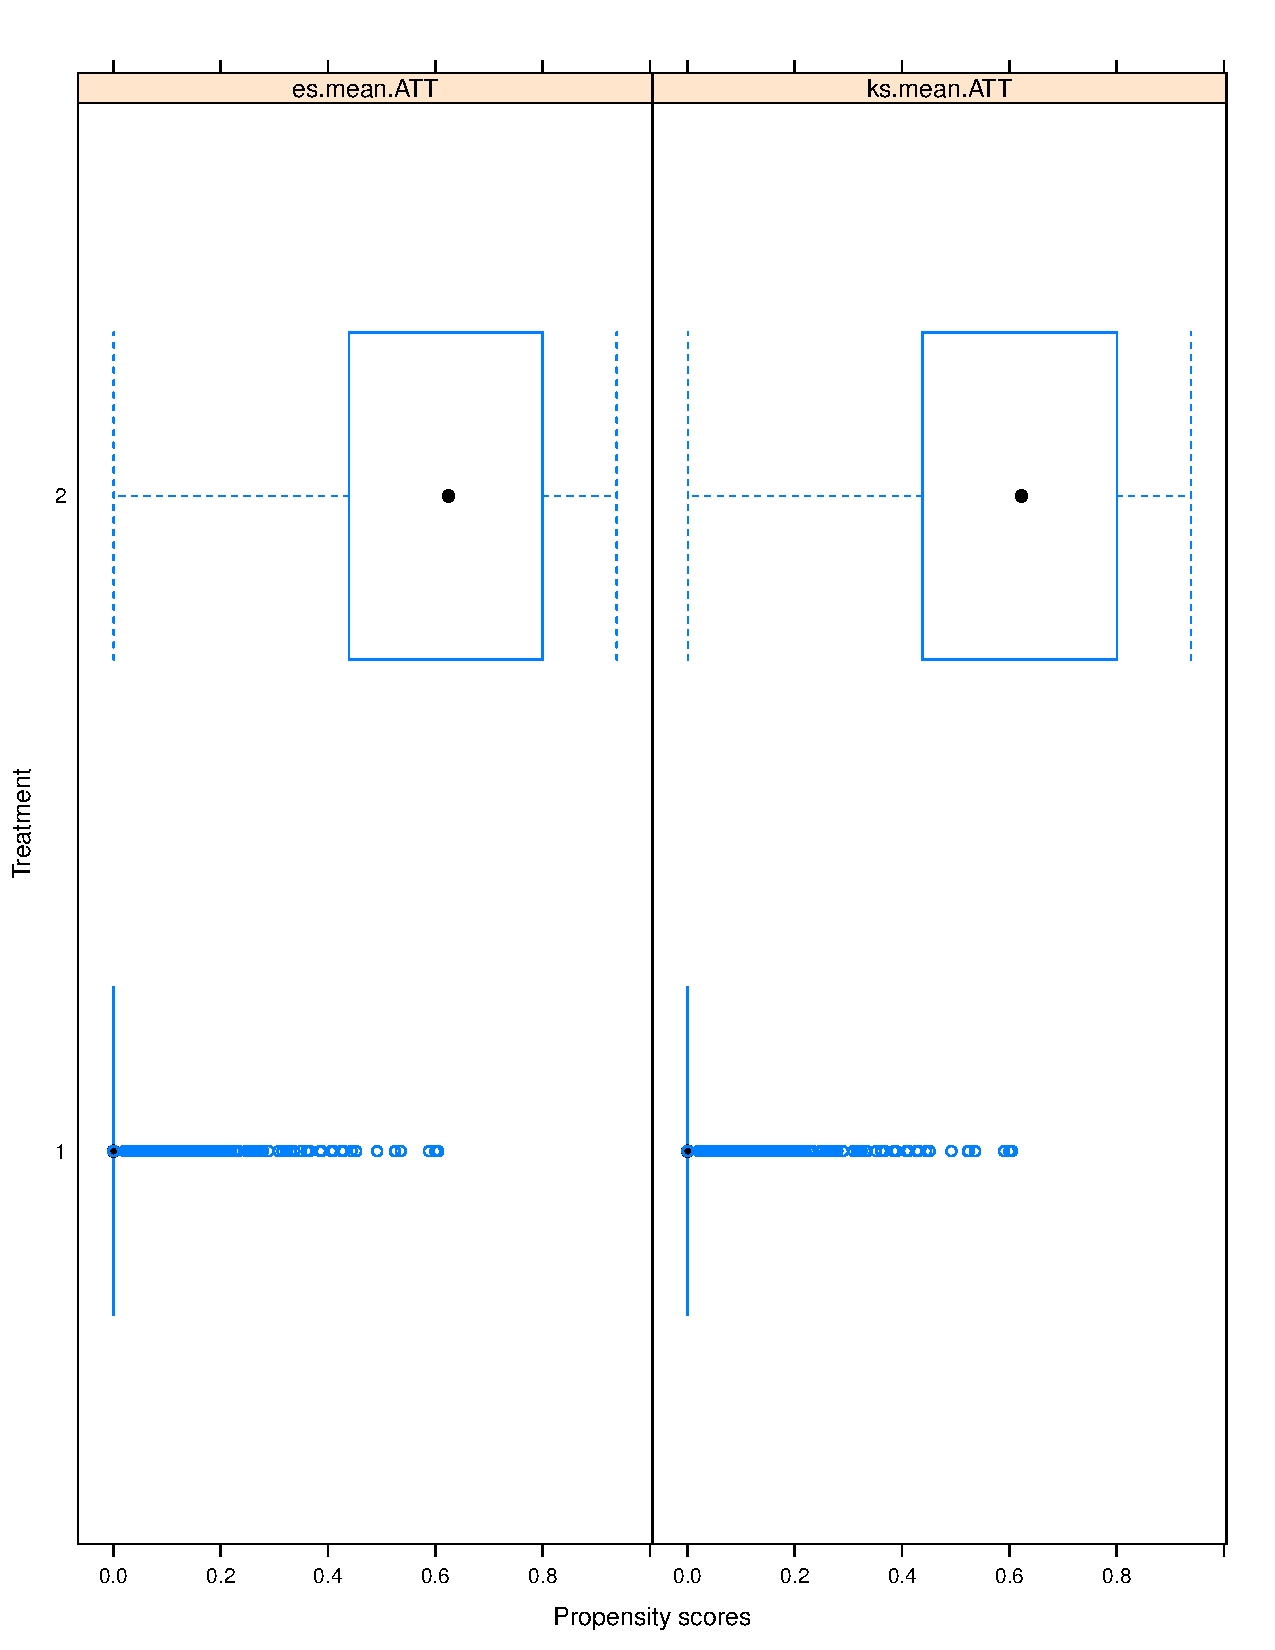
\includegraphics[scale=0.25]{./figs/psoverlap}
% where an .eps filename suffix will be assumed under latex, 
% and a .pdf suffix will be assumed for pdflatex; or what has been declared
% via \DeclareGraphicsExtensions.
\caption{Overlap of the estimated propensity scores between the non-GDP hours or control group (1 on y-axis) and the GDP hours treatment group (2 on the y-axis).  There is non-zero overlap as required for counterfactual estimation, and in particular there are hours in the control group that have propensity scores similar to the treatment group, implying similar weather and traffic covariates, and thus will be weighted more greatly by IPTW for estimating the counterfactual.  The subplots represent two different propensity score models fit with different criteria for optimal covariate balance (see appendix).}
\label{psoverlap}
\end{figure}
 
\subsection{Outcome Analysis}
As we have determined that our propensity score model leads to greater covariate balance as show in table \ref{tab:balance}, we can continue onwards to analyze the effect of treatment (GDP) on the outcome (airborne holding delay). Since the two groups are now balanced, the situation is similar to a RCT, and one can linearly regress the outcome simply on an indicator variable for treatment. Note that computationally one uses weighted linear regression with IPTW weights computed from the previously fitted propensity score models \cite{ridgeway2015toolkit}. After using this procedure we estimate the ATT, E(Y1$|$t=1)-E(Y1$|$t=0), to be $-1.4$ minutes.  In other words, had a GDP not been applied to the hours at JFK when it in fact was, the hourly average airborne delay would increase by 1.4 minutes (with a standard error of the same magnitude).  Although consistent with the common understanding that GDP reduces airborne delay, our results also indicate this difference is not statistically significant.  To further analyze this results, one can enlarge the sample size (recall we focused only on backdated GDP to avoid weather forecast uncertainty), but should also consider the possibility that GDP affected flights may receive additional en route airborne delay from additional TFMI \cite{bilimoria2016analysis}. 


%\begin{table}[h!]
%\begin{center}
%\begin{tabular}{|l|l|l|}
%\hline
%{\bf Acronym} & {\bf Name} & {\bf Notes}\\
%\hline
%TAF & Terminal Area/& Hourly summaries of forecast weather.\\
%\hline
%ASPM & FAA Aviation System & Hourly counts of scheduled and observed arrivals and\\
%& Performance Metrics & departures.\\
%& & Comprehensive historical archive available from FAA.\\
%\hline
%NTML & National Traffic & Description of implemented ATFMIs, including GDP.\\
%     & Management Logs & Comprehensive historical archive provided by NASA.\\
%\hline
%\end{tabular}
%\caption{Summary of relevant datasets required to apply Causal Inference to GDP decision making.}
%\end{center}
%\label{datasets}
%\end{table}






%\hfill mds
% 
%\hfill August 26, 2015

\section{Conclusion}
Our simplified application of causal inference served to illustrate a novel methodology to the ATM research community.  However in order to further validate results from such an analysis, namely counterfactual estimation of airborne delays from GDP, it would be useful to compare against simulations or queuing models.    

As demonstrated with a simplified constant capacity (service rate) queuing model in \cite{ball2001analysis}, the mean Airborne delay is a function of the ratio of PAAR and the arrival capacity,  subject to random fluctuations due to demand uncertainties, which increases when the PAAR exceeds the actual AAR\footnote{More complex queueing models of airborne delay are possible, as in \cite{gwiggner2014data}, which account for details of the three-dimensional arrival flows using radar data and subsequently employ non-homogenous queueing models to allow for temporal variations in arrival and service rates.  Non-Homogenous stochastic processes have been proposed as offering a better fit to observed airborne delay statistics \cite{caccavale2014model} when compared to the simpler, but often used, assumption of a Poissionian arrival process.}.  A direct comparison to such a queuing model would require casual analysis not with a binary treatment variable as we have, but rather a continuous treatment variable using empirical data to form the ratio of PAAR and arrival capacity (both available in ASPM).  We leave such modeling for future research, which can leverage more advanced propensity score estimation techniques for continuous treatment\footnote{See for example \cite{kreif2015evaluation} and references therein.}, which are relatively new.   A further anticipated complication with comparison to queuing models is that arrival capacity is also both dynamic and stochastic, while also influenced by departure demand \cite{jacquillat2015endogenous}. 

Furthermore, although we have chosen our unit of analysis to be an hour block of time, other units of analysis may also be possible.  For example, if one had access to flight level data, in terms of both outcomes (airborne delay) and treatment assignment (GDP induced ground delay ), it may be feasible to consider a single flight as the unit of analysis.  However again, the challenge with individual flight data will be to account for possibly additional TFMI that may increase the airborne delay to flights already subject to GDP, as hypothesized in \cite{bilimoria2016analysis}.  It may be difficult to account for en-route airborne delays, some of which may not be due TFMI at all, but rather due to Air Traffic Control actions, and thus requiring detailed radar data for analysis of actual flight trajectories \cite{belkoura2016generation}.  Determining if there is a systematic difference for GDP and non-GDP affect flights from these sources of additional airborne delays is a precursor to causal analysis that can account for such an imbalance to estimate counterfactual airborne delays.  

Even in our simplified setting of binary treatments, there are considerations that deserve further analysis.  Causal inference requires certain assumption be satisfied, including that all confounding variables that affect treatment and assignment have been measured \cite{austin2011introduction}.  Our modeling took into account certain meteorological and traffic covariates (\ref{tab:imbalance}), but it is well known that GDP can be implemented for other reasons, including maintenance events or large-scale disruptions to the NAS.  To what degree such an assumption is satisfied needs further investigation.  Another assumption of causal inference is that the potential outcome of a unit be unaffected by the treatment assignment of other units\footnote{This is called the stable unit treatment value assumption (SUTVA).}.  In our case such an assumption would require that the hourly average airborne delay be independent of GDP assignment of other hour blocks.  However there can be autocorrelation of airborne delay in neighboring hour blocks, based on whether those neighboring blocks are GDP or non-GDP hours.  Further analysis of such treatment dependent autocorrelation is required and may necessitate aggregation to larger blocks of hours or an entire day to satisfy the necessary assumption.  Such time-varying treatment assignment may also necessitate more advance Causal Inference methodology, which have been recently developed\cite{imai2015robust}. 

There also several possible extensions of our initial application of causal inference framework and methodology to ATM.  One is to simply consider how such a framework may apply to other TFMI besides GDP, using the language of treatment, outcomes, and propensity score analysis. Further extensions to the GDP context could include hourly analysis of the entire New York metro, using weather covariates from all airports simultaneously in multi-valued (but not continuous) treatment setting, where treatment corresponds to a categorical variable indicating GDP absence or presence at each of the major airports.  Another extension is to consider continuous valued treatments by explicitly considering the length of the ground-delay as the treatment variable, and estimating what in statistics is called the ``dose-response curve" \cite{kreif2015evaluation}, with airborne delay playing the role of the response.    






% An example of a floating figure using the graphicx package.
% Note that \label must occur AFTER (or within) \caption.
% For figures, \caption should occur after the \includegraphics.
% Note that IEEEtran v1.7 and later has special internal code that
% is designed to preserve the operation of \label within \caption
% even when the captionsoff option is in effect. However, because
% of issues like this, it may be the safest practice to put all your
% \label just after \caption rather than within \caption{}.
%
% Reminder: the "draftcls" or "draftclsnofoot", not "draft", class
% option should be used if it is desired that the figures are to be
% displayed while in draft mode.
%
%\begin{figure}[!t]
%\centering
%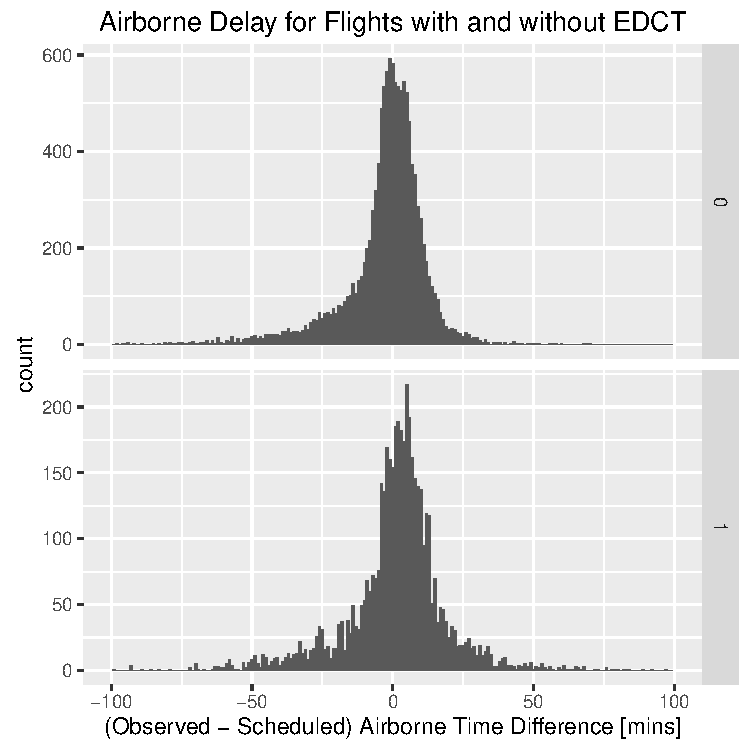
\includegraphics[scale=0.5]{abdiff_unw_faceted}
%% where an .eps filename suffix will be assumed under latex, 
%% and a .pdf suffix will be assumed for pdflatex; or what has been declared
%% via \DeclareGraphicsExtensions.
%\caption{Simulation results for the network.}
%\label{fig_sim}
%\end{figure}

\section{Appendix}
A model for the propensity score is a function from the space of covariates $X_i$ to $0<e_i=Pr(Z_i=1|X_i)<1$, or more traditionally to the log-odds $e_i$, namely:  
\begin{equation}
\log\frac{e_i}{1-e_i}=F(X_i)
\end{equation}
The most basic model for $F(X)$ is to assume linearity, $F(X)=\beta X$, which is then fit just as linear logistic regression models are\footnote{Notice that we are regressing the covariates $X_i$ on the log-odds of the probability of treatment $e_i$, and \emph{not} on the outcomes directly.}. However this simplest linear model has been shown in simulation and actual studies to not achieve the best balance between treatment and control covariates .  

We note here that previous ATM research has also used linear logistic regression to model the probability of a GDP occurring, with a goal of fitting the most accurate GDP classifier to ultimately identify similar weather impacted airport days \cite{Grabbe:2014aa}.  However we emphasize that our goal is \emph{not} to derive the most accurate classifier but instead to use the probability of a GDP (or other TFMI) occurring as a balancing score for counterfactual estimation, and thus even if we employed linear logistic regression, the optimal model coefficients obtained using metrics for balance, would certainly be different that those using metrics for accurate classification.

More robust alternatives to linear logistic models for propensity score include machine learning methods \cite{lee2010improving}, such as Generalized Boosted Models (GBM), which employ combinations of non-parametric piecewise-linear functions that adapt to the data and are thus more flexible than a linear model.  In addition GBM is implemented in open-source statistical software \cite{ridgeway2006gbm} and can thus be easily replicated by other researchers.  Furthermore, when GBM is used as the model for propensity score, fitting procedures which employ optimization to tune these piecewise linear functions to achieve best balance between treatment and control covariates are also readily implemented in open-source statistical software \cite{ridgeway2015toolkit}.  Furthermore there are various quantitative balance metrics that can be easily accessed to assess the quality of the resultant propensity score model \cite{ridgeway2015toolkit}. 

Once the propensity score model has been fit, one can use the resulting propensity scores for each subject, $e_i$, to balance the covariates $X_i$ between treatment and control groups and thereby reduce or eliminate confounding.  The four principal methods to reduce confounding using propensity scores are: matching, stratification, inverse probability of treatment weighting (IPTW), and covariate adjustment \cite{austin2011introduction}.  We will only summarize IPTW as it has been thoroughly implemented and tested in software \cite{ridgeway2015toolkit}, and has also been extended to multiple treatments \cite{mccaffrey2013tutorial}, which will eventually be required if we want to consider the effect of various TFMI options beyond just ``GDP or no-GDP."  Previous research on TFMI \cite{tfmiCluster} has shown there are likely many categories of TFMI that occur and which combine the various courses of actions available to decision makers, each with their own specific operational parameters. Thus extensions of propensity score modeling beyond binary treatments is a desirable property of IPTW.

Recall that $Z_i$ is an indicator variable which denotes treatment status, i.e. $Z_i=1$ if the subject received treatment.  IPTW defines weights for each subject that capture the inverse probability the subject received treatment as follows \cite{austin2011introduction}:

\begin{equation}
w_i = \frac{Z_i}{e_i} + \frac{1-Z_i}{1-e_i}.
\end{equation}
The intuition behind the weights is the following: those subject in the control group ($Z_i=0$) whose propensity scores (probability of being selected for treatment) are relatively higher ($e_i$ is  larger) are ``weighted up" and thus their covariates are more greatly weighted when assessing balance after weighting.  Various balance measures after weighting with $w_i$ are possible using significance testing for differences of means, medians, variance, and Kolmogorov-Smirnov statistics\cite{ridgeway2015toolkit}.   

These weights can also be used to adjust the outcome for each subject $Y_i$ and thereby simulate counterfactuals used to estimate ATT or ATE.  For example to estimate ATT, one weights the outcomes (e.g. airborne delay) for the treatment group with unity and for the control group with weights $w_i=e_i/(1-e_i)$.  Then the ATT treatment effect $E(Y_i(Z_i=1)-Y_i(Z_i=0)|Z_i=1)$ can be estimated by regressing on a single variable, the treatment indicator \cite{ridgeway2015toolkit}, or in the simplest model by arithmetic mean of the weighted counterfactual outcome.  


\subsection{Advantages of propensity score over regression to reduce confounding}
As explained in \cite{mccaffrey2013tutorial}, there are several reasons why propensity score techniques are advantageous over such regression-based techniques and here we simply summarize these advantages:

\begin{itemize}
\item \emph{dimensional reduction}: propensity scores summarize all covariates into a single score and act as an important dimensional reduction tool for evaluating treatment effects. Whereas regression methods require specifying a model that depends on all covariates (and various interactions).

\item  \emph{grounded in rigorous framework}: propensity score methods derive from a formal statistical model for causal inference, the potential outcomes framework, so that causal questions can be well-defined and explicitly specified and not conflated with the modeling approach as they are with traditional regression approaches

\item  \emph{robust against model misspecifcation}: propensity score methods do not require modeling the mean for the outcome, which can help avoid bias from misspecification of that model 

\item \emph{avoid extrapolation}: propensity score methods avoid extrapolating beyond the observed data unlike parametric regression modeling for outcomes which extrapolate whenever the treatment and control groups are disparate on pretreatment variables

\item \emph{propensity score adjustments} (e.g. IPTW weights) can be determined using only the pretreatment covariates and treatment assignments, eliminating the influence that estimated treatment effect can have on model specification of covariates.
\end{itemize}

% Note that the IEEE typically puts floats only at the top, even when this
% results in a large percentage of a column being occupied by floats.


% An example of a double column floating figure using two subfigures.
% (The subfig.sty package must be loaded for this to work.)
% The subfigure \label commands are set within each subfloat command,
% and the \label for the overall figure must come after \caption.
% \hfil is used as a separator to get equal spacing.
% Watch out that the combined width of all the subfigures on a 
% line do not exceed the text width or a line break will occur.
%
%\begin{figure*}[!t]
%\centering
%\subfloat[Case I]{\includegraphics[width=2.5in]{box}%
%\label{fig_first_case}}
%\hfil
%\subfloat[Case II]{\includegraphics[width=2.5in]{box}%
%\label{fig_second_case}}
%\caption{Simulation results for the network.}
%\label{fig_sim}
%\end{figure*}
%
% Note that often IEEE papers with subfigures do not employ subfigure
% captions (using the optional argument to \subfloat[]), but instead will
% reference/describe all of them (a), (b), etc., within the main caption.
% Be aware that for subfig.sty to generate the (a), (b), etc., subfigure
% labels, the optional argument to \subfloat must be present. If a
% subcaption is not desired, just leave its contents blank,
% e.g., \subfloat[].


% An example of a floating table. Note that, for IEEE style tables, the
% \caption command should come BEFORE the table and, given that table
% captions serve much like titles, are usually capitalized except for words
% such as a, an, and, as, at, but, by, for, in, nor, of, on, or, the, to
% and up, which are usually not capitalized unless they are the first or
% last word of the caption. Table text will default to \footnotesize as
% the IEEE normally uses this smaller font for tables.
% The \label must come after \caption as always.
%
%\begin{table}[!t]
%% increase table row spacing, adjust to taste
%\renewcommand{\arraystretch}{1.3}
% if using array.sty, it might be a good idea to tweak the value of
% \extrarowheight as needed to properly center the text within the cells
%\caption{An Example of a Table}
%\label{table_example}
%\centering
%% Some packages, such as MDW tools, offer better commands for making tables
%% than the plain LaTeX2e tabular which is used here.
%\begin{tabular}{|c||c|}
%\hline
%One & Two\\
%\hline
%Three & Four\\
%\hline
%\end{tabular}
%\end{table}


% Note that the IEEE does not put floats in the very first column
% - or typically anywhere on the first page for that matter. Also,
% in-text middle ("here") positioning is typically not used, but it
% is allowed and encouraged for Computer Society conferences (but
% not Computer Society journals). Most IEEE journals/conferences use
% top floats exclusively. 
% Note that, LaTeX2e, unlike IEEE journals/conferences, places
% footnotes above bottom floats. This can be corrected via the
% \fnbelowfloat command of the stfloats package.





% conference papers do not normally have an appendix


% use section* for acknowledgment
\section*{Acknowledgment}


The author would like to thank Heather Arneson, Paul Lee, Anthony Evans, and Karl Bilimoria of NASA Ames for useful correspondence and feedback.  We also thank our colleagues Matthew Cefalu and Beth Ann Griffin of the RAND Center for Causal Inference for fruitful discussions.  In addition we thank Kenneth Kuhn, Christopher Skeels, and Kyle Murray for collaboration on related research.






% trigger a \newpage just before the given reference
% number - used to balance the columns on the last page
% adjust value as needed - may need to be readjusted if
% the document is modified later
%\IEEEtriggeratref{8}
% The "triggered" command can be changed if desired:
%\IEEEtriggercmd{\enlargethispage{-5in}}

% references section

% can use a bibliography generated by BibTeX as a .bbl file
% BibTeX documentation can be easily obtained at:
% http://mirror.ctan.org/biblio/bibtex/contrib/doc/
% The IEEEtran BibTeX style support page is at:
% http://www.michaelshell.org/tex/ieeetran/bibtex/
\bibliographystyle{IEEEtran}
% argument is your BibTeX string definitions and bibliography database(s)
\bibliography{IEEEabrv,./gdp_causal}
%
% <OR> manually copy in the resultant .bbl file
% set second argument of \begin to the number of references
% (used to reserve space for the reference number labels box)
%\begin{thebibliography}{1}
%
%\bibitem{IEEEhowto:kopka}
%H.~Kopka and P.~W. Daly, \emph{A Guide to \LaTeX}, 3rd~ed.\hskip 1em plus
%  0.5em minus 0.4em\relax Harlow, England: Addison-Wesley, 1999.
%
%\end{thebibliography}
\vspace*{-35\baselineskip}

 \begin{IEEEbiography}[\centerline{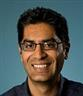
\includegraphics[width=10in,height=10.25in,keepaspectratio]{./figs/ashah}}]{Akhil Shah}
%\begin{IEEEbiographynophoto}{Akhil Shah}

is a Senior Engineer with the RAND Corporation where he develops machine learning and statical methodology for air-traffic and cybersecurity related research problems.  He received his PhD in Theoretical High Energy Physics and M.S. in Electrical Engineering from UCLA.  His previous research involved communication system design and analysis for both wireless and optical applications.  
 \end{IEEEbiography}
%\end{IEEEbiographynophoto}



% that's all folks
\end{document}


